\chapter{Knowledge Distillation}
\label{part_2}
Frugal \acrshort{ai} is an emerging concept that aims to develop models capable of "doing more with less". Frugal models consume less resources while providing great results. \acrshort{kd} is a frugal \acrshort{ai} technique that consists in using the results of a large model to help a smaller model during its training. This model's performance tends towards that of the large model. This research work focuses on applying \acrshort{kd} to \acrshort{lic}. Usually, KD is accomplished by training a small model (student) on the output of a well performing large model (teacher). For classification task, the student will have to reproduce the output softmax probabilities of the teacher. This way, the student does not only learn to predict the correct class but also which classes are similar. Following the same reasoning, it makes sense to apply KD to the output of both the encoder and the decoder. The former will assist the student in finding a good latent representation and the latter will help the student to reconstruct input images. This chapter focuses on applying \acrshort{kd} to \acrshort{lic}. In order to do that, we first experiment with \acrshort{kd} on auto-encoders for image reconstruction. After achieving satisfactory results, we proceed in implementing \acrshort{kd} for \acrshort{lic}.

\section{Knowledge Distillation for Image Reconstrution}
As discussed by Ballé et al. in \cite{ballé2018variationalimagecompressionscale}, \acrfull{vae} share similarities with \acrshort{lic} architectures. Both use an analysis transformation to map the input signal to a lower-dimensional latent space, followed by an approximate inverse transformation (the synthesis transform) to map the latent representation back to the signal space. However, as highlighted by Minnen et al. in \cite{minnen2018jointautoregressivehierarchicalpriors}, there is a key distinction between the two approaches. Compression is not just about reducing dimensionality; it involves reducing the entropy of the representation under a prior probability model that is shared between the sender and the receiver. Achieving high-performance image compression is, therefore, more complex than merely reconstructing images.

In this study, we explore the application of \acrshort{kd} to auto-encoders for image reconstruction, which is a more straightforward task than image compression. Initially, we familiarize ourselves with this technique by implementing it on custom-built \acrfull{ae}. Subsequently, we apply the same technique to state-of-the-art image compression models that are used as \acrshort{ae}s.

\subsection{Custom Auto-encoder}
This experiment investigates the application of \acrshort{kd} on well-established architectures, such as convolutional \acrshort{ae}s, and evaluates the impact of \acrshort{kd} on performance. Specifically, we train a large model (the teacher) and a smaller model (the student) both with and without \acrshort{kd}. We expect the student model, when trained with \acrshort{kd}, to achieve superior image reconstruction performance compared to the other small model. Ideally, the student model would achieve results comparable to those of the teacher model.

We design the teacher encoder with three stages each containing two convolutions with ReLU followed by a maximum pooling. This is followed by a two-layer fully connected network to achieve a latent space size of 256. The teacher decoder follows the same structure but reversed with transpose convolutions instead of convolutions and up-sampling to replace pooling. The small architecture is analogous with only one convolution (or transpose convolution) per stage. The student model is trained based on its output (by comparing the input and output images using \acrshort{mse}) but also based on the latent representation and the output of the teacher model (using \acrshort{mse} for both).

Exposed in Figure \ref{kd_ae_test_1} are the first results obtained. While mediocre in terms of \acrshort{kd} effectiveness, they highlight the importance of the "quality" of the teacher. Continuing the analogy of the teacher and student relationship, it makes sense that a good teacher is more likely to train a good student than a bad teacher. In the context of \acrshort{kd}, the student learns partially from the output of the teacher, so we must use a powerful teacher network, otherwise the student network will learn poor latent representations as well as reconstructions. In order to achieve the best possible results, we decide to perform the upcoming experiments using pre-trained networks from the compressAI model zoo as teachers. On top of dramatically reducing the training time for each experiment, it also allow us to easily compare our models to state-ot-the-art results.

\begin{figure}
    \centering
    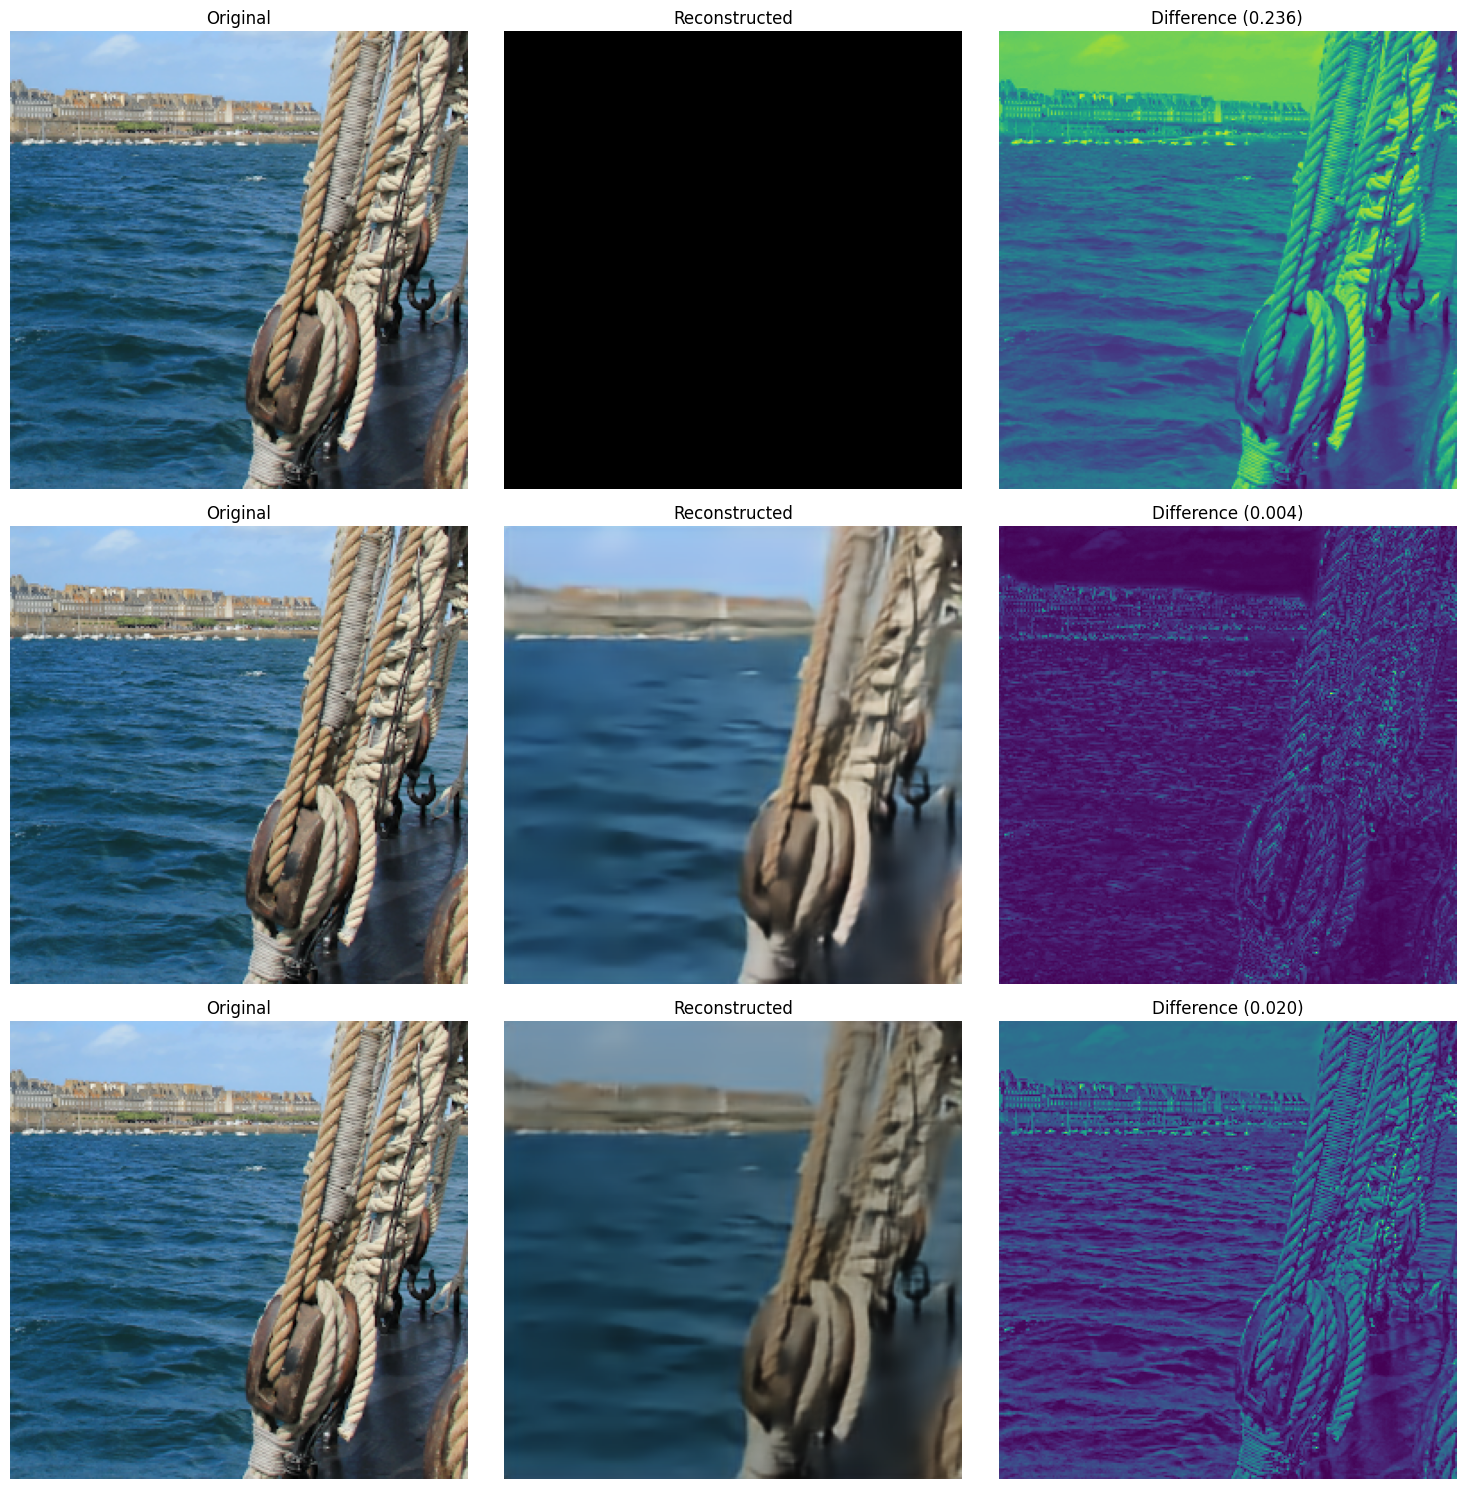
\includegraphics[width=8cm]{../img/kd_ae_test_1.png}
    \caption[Image reconstruction comparison of teacher and student architectures.]{Image reconstruction comparison of teacher and student architectures. In this experiment, the teacher (top row) converged to a degenerate solution. The student architecture without \acrshort{kd} (middle row) did not collapse and reach a \acrshort{mse} of 0.004 on this sample. When trained by the underperforming teacher, the student architecture (bottom row) suffers a performance loss: the \acrshort{mse} increases to 0.020. The impact of \acrshort{kd} is very noticable: the reconstructed image lacks details and is darker.}
    \label{kd_ae_test_1}
\end{figure}

\subsection{Scale Hyperprior Model as Auto-encoder}
\label{scale_hyperprior_ae}
Building on the previous section, which highlighted the benefits of \acrshort{kd} for auto-encoders, we now turn our attention to applying this technique to image compression. With this in mind, we take a step-by-step approach, beginning with an attempt to observe similar results using architectures designed for image compression. The objective of the following experiment is to employ the state-of-the-art scale hyperprior model as an \acrshort{ae} for image reconstruction. As mentioned earlier, image reconstruction closely resembles image compression, but without the entropy constraint on the latent space. Since the scale hyperprior model is designed for \acrshort{lic}, we expect it to perform well on this less challenging task.\footnote{An additional benefit of this experiment is that it provides a code foundation for following experiments focused on \acrshort{lic}.}

The following experiment consists in training five students models with different architectures. Using the pre-trained scale hyperprior model optimised for \acrshort{mse} with \textsf{quality} set to 5 (with 128 channels and a latent space of size 192) as teacher, we train models with different number of channels. We define five models with 16, 32, 64, 96 and 112 channels (symbolised by the parameter N in Figure \ref{scale_hyperprior_1:b}) while preserving the size of the latent space. We use the following \acrshort{kd} loss function:

\begin{equation}
    L = \lambda_{1}\, MSE(\hat{y}_{student}, \hat{y}_{teacher}) + \lambda_{2}\, MSE(\hat{x}_{student}, \hat{x}_{teacher}) + \lambda_{3}\, MSE(\hat{x}_{student}, x)
    \label{loss_1}
\end{equation}

We use the following set of parameters: \(\{\lambda_{1}, \lambda_{2}, \lambda_{3}\} = \{0.2, 0.2, 0.6\}\) and train the models with the method defined in Section \ref{training_method}: 1000 epochs on the Vimeo90K dataset with a base learning rate of \(10^{-4}\).

Figure \ref{kd_ae_1:a} shows reconstructions of image 14 of the Kodak dataset with the teacher and all student networks. As axpected, the teacher (a pre-trained model) propose a reconstructed image virtually undistinguishable from the orignal one. As for the students, eventhough they give visually satisfying results, the models with less parameters do not retain as much details. The reconstructed image appears a little bit blurry. As expected, the more the student architecture is similar to the teacher (that is to say, more channels), the more it is able to reach the same performance as the teacher. This is quantitatively measured using MSE on Figure \ref{kd_ae_1:b}.

\begin{figure}[H]
    \centering
    \subfloat[Reconstruction results on image 14 of the Kodak dataset with teacher and student architectures.]{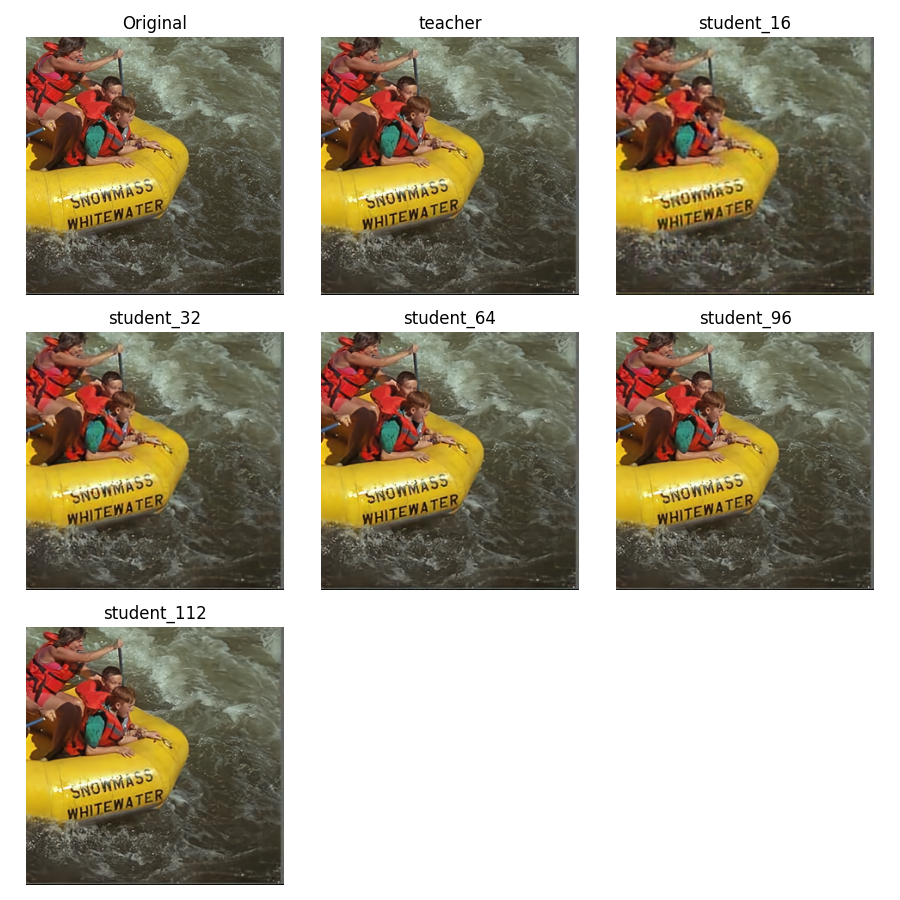
\includegraphics[width=8cm]{../img/kd_ae_kodak_14.png} \label{kd_ae_1:a}}
    \qquad
    \subfloat[Average \acrshort{mse} curve on the Kodak dataset for students with different number of channels.]{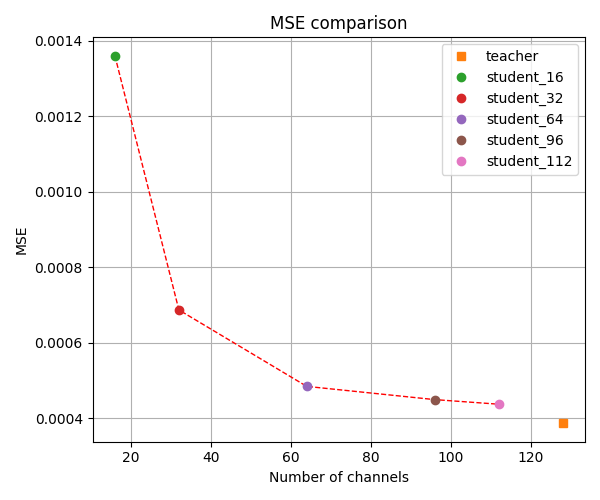
\includegraphics[width=8cm]{../img/kd_ae_mse.png} \label{kd_ae_1:b}}
    \caption[Evaluation on the Kodak dataset of the scale hyperprior student models trained for image reconstruction.]{Evaluation on the Kodak dataset of the scale hyperprior student models trained for image reconstruction. Student models with fewer channels propose less detailed image reconstruction. This is noticeable on single image reconstructions or on average using \acrshort{mse} measures.}
    \label{kd_ae_1}
\end{figure}

For reference, we show in Figure \ref{kd_ae_2} the \acrshort{rd} performance of the student models. It should be noted that the teacher network used in this experiment was trained for image compression tasks so one could argue that these models are not exactly auto-encoders for image reconstruction. What is sure is that they are far from state-of-the-art models in image compression tasks. What remains to be seen is to what extent a properly defined \acrshort{kd} loss for \acrshort{lic} does increase the \acrshort{rd} performance of these student models. This, as well as discussion related to the benefits of smaller student models for \acrshort{lic}, is the subject of the next section.

\begin{figure}
    \centering
    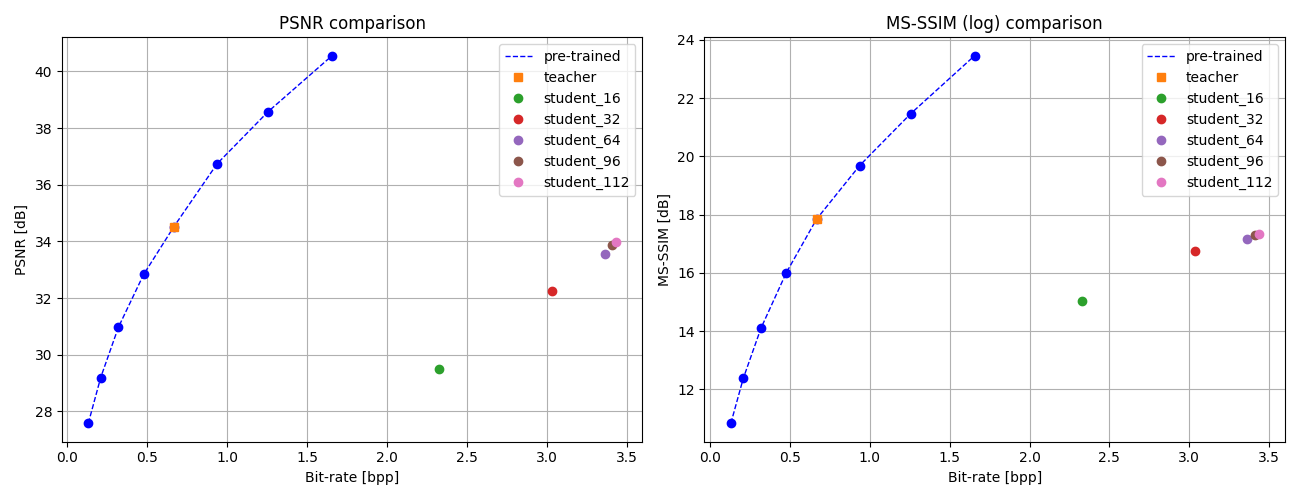
\includegraphics[width=15cm]{../img/kd_ae_rd.png}
    \caption[Average \acrshort{rd} performance on the Kodak dataset for students with different number of channels.]{Average \acrshort{rd} performance on the Kodak dataset for students with different number of channels. Eventhough they were guided by a \acrshort{lic} model during their training, the student models poorly compares to state-of-the-art models in \acrshort{rd}. (The pre-trained models are compressAI scale hyperperior models with \extsf{quality} from 1 to 8).}
    \label{kd_ae_2}
\end{figure}

Whether it is for custom convolutional \acrshort{ae} or models specifically designed for \acrshort{lic}, there is no denial that \acrshort{kd} positively influence the performance of small models. This section certify this result for image reconstruction, we now transfer this technique to \acrshort{lic} domain.

\section{Knowledge Distillation for Image Compression}
Having assessed the effectiveness of \acrshort{kd} for computer vision tasks similar to image compression, we investigate the success of this frugal \acrshort{ai} technique on \acrshort{nn}-based image compression. Still using the scale hyperprior model introduced in \cite{ballé2018variationalimagecompressionscale}, we train a serie of student models with \acrshort{kd} to evaluate both their \acrshort{rd} performance and their ability to be deployed on resource constrained platforms.

\subsection{Rate-Distortion Performance}
This section aims at evaluating the \acrshort{rd} performance gain achievable through \acrshort{kd}. By guiding small models during their training with a teacher model, we hope to increase their ability to compress images. We first explain our method then we present our results.

\subsubsection{Method}
\acrshort{lic} distinguish itself from other computer vision tasks (such as dimensionality reduction) by minimising the entropy of the latent representation. In dimensionality reduction, the latent representation has no practical application. When it comes to image compression, it is the latent representation of the image that will be stored or transmitted. Having the smallest possible entropy allows for a smaller entropy coding which means less bits to handle in real world applications. This is why the rate-distortion loss is used in \acrshort{lic} as it allows to find a tradeoff between image quality and bit rate according that fits the requirements of the application. In order to have similar results with \acrshort{lic}, the previous loss function, introduced in Equation \eqref{loss_1}, is updated as follow:

\begin{align}
    L = \lambda_{1}\, MSE(\hat{y}_{student}, \hat{y}_{teacher}) + \lambda_{2}\, MSE(\hat{x}_{student}, \hat{x}_{teacher}) + \lambda_{3}\, RD(\hat{y}_{student}, \hat{x}_{student}, x)\label{loss_2}\\
    RD(\hat{y}_{student}, \hat{x}_{student}, x) = -E[\log_{2}\hat{y}_{student} + \log_{2}\hat{z}_{student}] + \lambda\, MSE(\hat{x}_{student}, x)
\end{align}

We also tried to use the Kullback-Leibler divergence instead of \acrshort{mse} loss function on the latent space but found that it resulted in slightly higher bit rates. Outcome of this experiment is exposed in Figure \ref{appendix:kd_lic_1_kld}.

For easier comparison and because our study focuses on low bit rate image compression, we compare our results to compressAI pre-trained models with \textsf{quality} from 1 to 5.

\subsubsection{Architecture Size Tradeoff}
\label{architecture_size_tradeoff}
The objective of \acrshort{kd} is to improve the performance of small models using a large one. However, there is no definition of "a small model" so we start by experimenting with model sizes. Following our training method, we create five new models using \acrshort{kd} and the loss function from Equation \ref{loss_2}. We use \(\lambda = 0.025\) in the \acrshort{rd} part of the loss, the same value used by the teacher model during its training. The five models have different sizes. We modify their architecture by changing the number of channels. The smallest deals with as few as 16 channels while the largest student has 112 (number of channels is indicated by the parameter N in Figure \ref{scale_hyperprior_1:b}). It should be noted that the size of the latent space remains the same across all models, teacher and students.

Unsurprisingly, using \acrshort{RD} loss yields far better results for image compression. Contrary to similar models trained with \acrshort{mse} only (Section \ref{scale_hyperprior_ae}), these new models can be found in the same operational \acrshort{rd} area as state-of-the-art models (Figure \ref{kd_lic_1}).

Results depicted in Figure \ref{kd_lic_1} follow our intuition. Students with larger number of channels (i.e. 64, 96 and 112) take full advantage of \acrshort{kd} and reach roughly the same \acrshort{bpp} and \acrshort{psnr} as the teacher. Models with 16 and 32 channels cannot reach the same level of image quality. Both of them end up far behind pre-trained models in \acrshort{rd} performance and results in higher \acrshort{mse} error (Figure \ref{kd_lic_2:b}). Eventhough they produce visually impressive results (Figure \ref{kd_lic_2:a}) for models with so few parameters, they are not relevant candidates when taking into account only \acrshort{rd} performance. The number of channels definitely impact the output quality in extreme scenarios (e.g. very few channels) but can be reduced to some extend without degrading image quality.

\begin{figure}
    \centering
    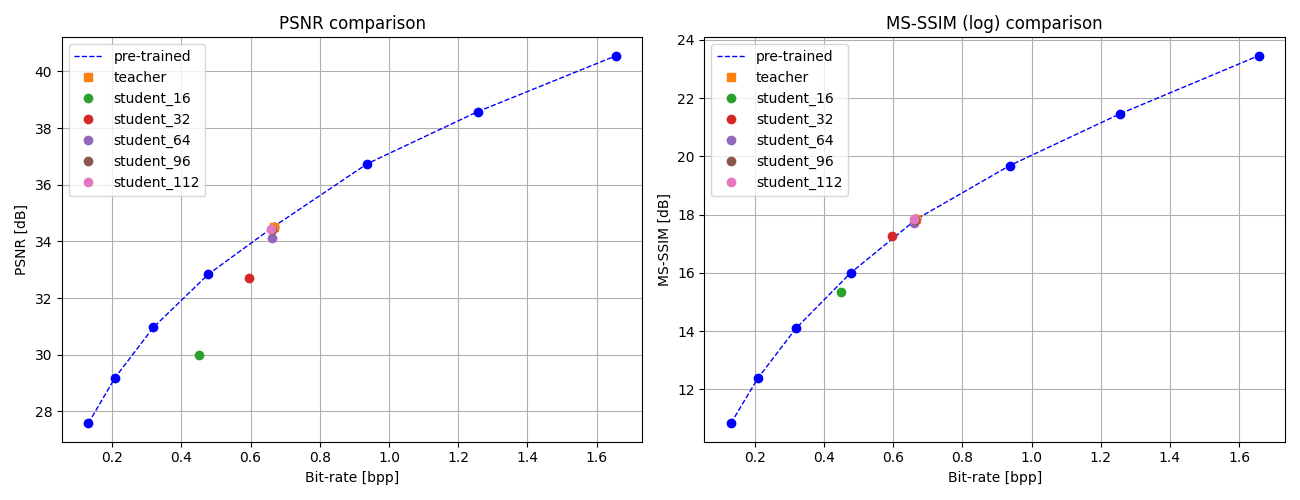
\includegraphics[width=15cm]{../img/kd_lic_rd_channels.png}
    \caption[Average \acrshort{rd} curve on the Kodak dataset for students with different number of channels.]{Average \acrshort{rd} curve on the Kodak dataset for students with different number of channels. Despite being trained similarly, all models have different outputs. Models with at least 64 channels performs alike their teacher but 16 and 32 channels are not sufficient to preserve the same image quality.}
    \label{kd_lic_1}
\end{figure}
% Use 263674, 274457, 274461, 274464, 263691

\begin{figure}[H]
    \centering
    \subfloat[Reconstruction results on image 14 of the Kodak dataset with teacher and student architectures.]{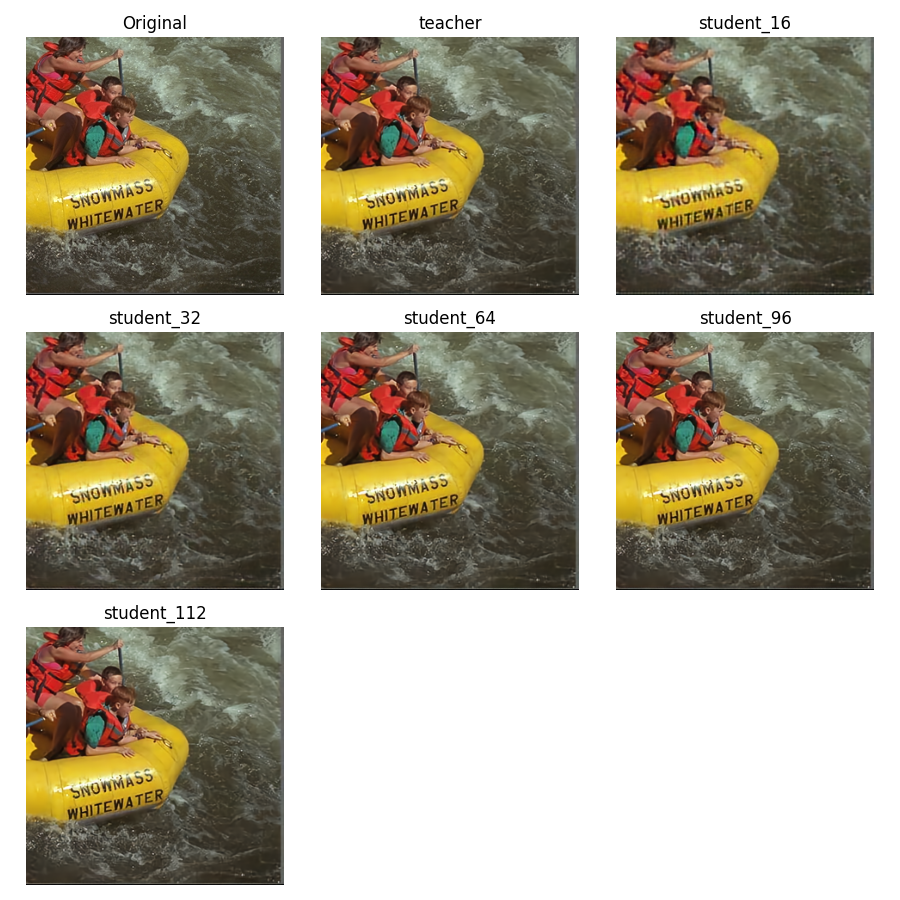
\includegraphics[width=8cm]{../img/kd_lic_kodak_14.png} \label{kd_lic_2:a}}
    \qquad
    \subfloat[Average MSE curve on the Kodak dataset for students with different number of channels.]{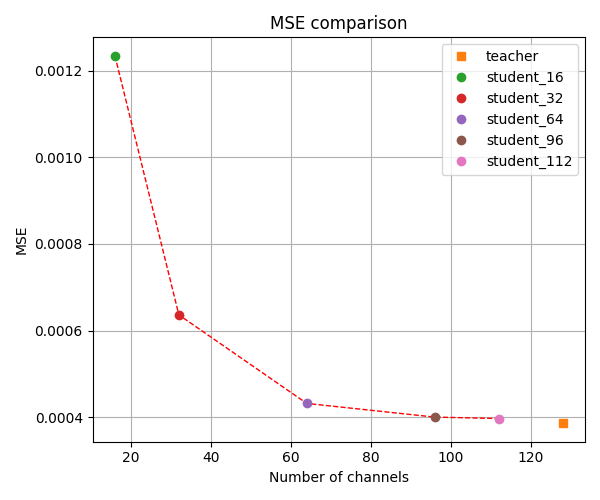
\includegraphics[width=8cm]{../img/kd_lic_mse.png} \label{kd_lic_2:b}}
    \caption[Evaluation on the Kodak dataset of the scale hyperprior student models trained for image compression.]{Evaluation on the Kodak dataset of the scale hyperprior student models trained for image compression. Meticulous visual inspection and average \acrshort{mse} of the output prove the importance of the number of channels when limiting compression loss.}
    \label{kd_lic_2}
\end{figure}

\subsubsection{Rate-Distortion Tradeoff}
Once again, following our training method, we train five new models using \acrshort{kd} and the loss function from Equation \ref{loss_2}. The teacher model is still taken from the compressAI zoo with \textsf{quality} set to 5. This time, we fix the number of channels across all models (i.e. 64, the smallest number of channels that did not degrade too much performance in previous experiments) but we use different values of \(\lambda\) in the \acrshort{rd} part of the loss. For easier comparison and because our study focuses on low bit rate image compression, we use the values of \(\lambda\) corresponding to the five lowest values of \textsf{quality} (Table \ref{tab_quality_lambda}). We use the pre-trained models corresponding to the same values of \(\lambda\) as a baseline to compare our results.

As a reminder, the pre-trained models in Figure \ref{kd_lic_4} all have 128 channels. This means that our student models all have half as many channels as the pre-trained models do. Still, all students have similar or higher \acrshort{psnr} than their pre-trained counter-part. More precisely, when quality is prioritised (student 4 and 5), \acrshort{kd} is not the ideal solution: the models performs better than what they would have if trained alone but they are restrained by the modest number of channels. Student 5 attain the limit of what is feasible with 64 channels: with the same \acrshort{rd} tradeoff as the teacher, it is not able to match the teacher image quality. However, smaller models (student 1, 2 and 3) trained to prioritise bit rate reach better \acrshort{psnr} thanks to the teacher model (trained to favorise image quality) pulling them toward the top of the chart. Another interesting experiment is to use a teacher trained to prioritize bit rate. In that case, we observe that all students are pushed toward the bottom left of the chart (Figure \ref{kd_lic_4_bis}). This compromise could be useful for storage or bandwidth critical operations.

\begin{figure}
    \centering
    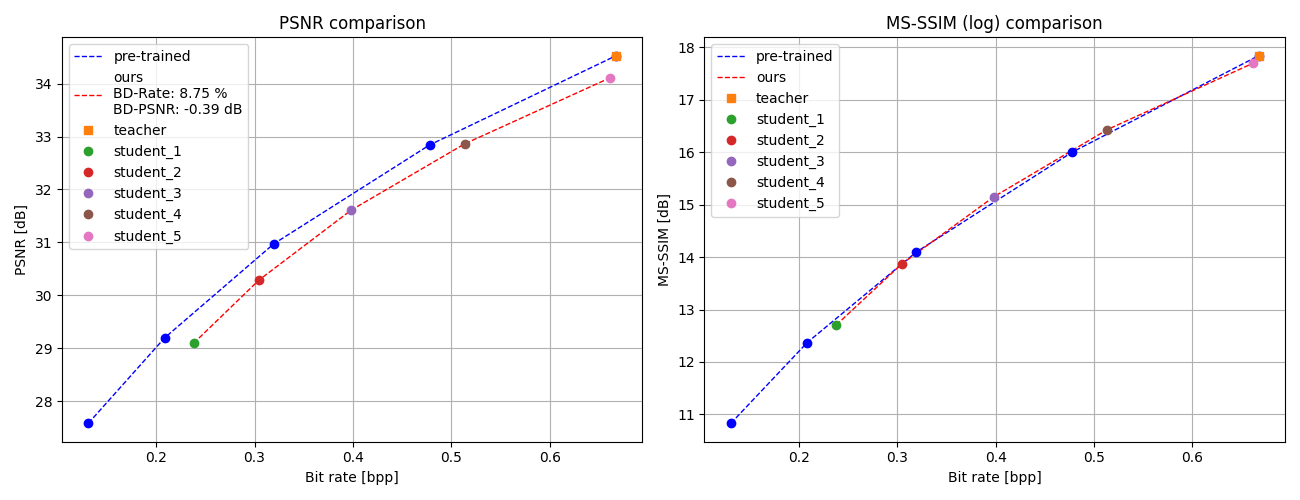
\includegraphics[width=15cm]{../img/kd_lic_rd_lambda_1.png}
    \caption[Average \acrshort{rd} curve on the Kodak dataset for students with different \acrshort{rd} tradeoffs.]{Average \acrshort{rd} curve on the Kodak dataset for students with different \acrshort{rd} tradeoffs. Trained by a teacher with an emphasis on image quality, students 1, 2 and 3 achieve better \acrshort{psnr} than their pre-trained counterpart. Students 4 and 5 are held back by the limited number of channels.}
    \label{kd_lic_4}
\end{figure}
% Use 280392, 281662, 281976, 281979, 274461

\begin{figure}
    \centering
    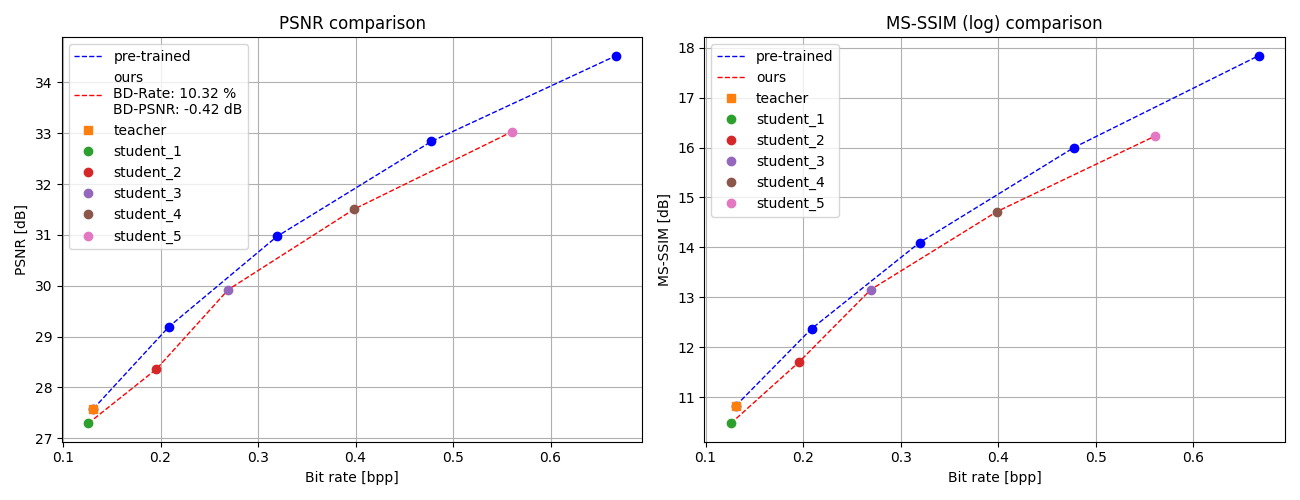
\includegraphics[width=15cm]{../img/kd_lic_rd_lambda_2.png}
    \caption[Average \acrshort{rd} curve on the Kodak dataset for students with different \acrshort{rd} tradeoffs and a teacher focusing on minimising bit rate.]{Average \acrshort{rd} curve on the Kodak dataset for students with different \acrshort{rd} tradeoffs and a teacher focusing on minimising bit rate. Student \acrshort{nn}s, influenced by they teacher at training time, have a lower bit rate than their pre-trained counterpart. The gap becomes more noticeable as \(lambda\) increases. This gain in bit rate implies a loss in image quality across all students.}
    \label{kd_lic_4_bis}
\end{figure}
% Use 289751, 295889, 289745, 296544, 289742

This section proves that \acrshort{kd} can be successfully applied to \acrshort{lic} tasks. We are able to train small models with \acrshort{rd} performance almost on par with larger models. But \acrshort{rd} performance is only one part of the equation with frugal \acrshort{ai}: we now need to assess the resource savings. It remains to be seen if it is worth making the tradeoff of loosing some \acrshort{rd} performance to use smaller models.

\subsection{Application to Resource Constrained Platfroms}
\label{application_resource_contrained_platforms}
Real life applications for \acrshort{lic} do not only focus on \acrshort{rd} performance. It is important to ensure great image quality at the lowest bit rate possible but other parameters need to be taken into account. Having proved the effectiveness of \acrshort{kd} for \acrshort{lic} tasks in terms of \acrshort{rd} performance with small student models almost on par with larger models, we now need to put into perspective these results. Let us dive into the second apsect of this study: making \acrshort{lic} possible on resource-limited platforms. This section analyses student models with different architectures from a resource stand point across three main axis: memory, computing power and energy consumption.

In this section, we use the models first introduced in Section \ref{architecture_size_tradeoff}. There are five student architectures with 16, 32, 64, 96 and 112 channels and a latent space of size 192. We compare our models to pre-trained models from the compressAI zoo (with \textsf{quality} ranging from 1 to 5).

Most resource constrained computers deal with a limited amount of memory. This limiting factor sometimes makes them unsuitable for tasks requiring large models. In \acrshort{lic}, distillation allows to use smaller models without degrading \acrshort{rd} performance. Our student models can have as few as 0.27 M parameters while standard models have 5 M parameters. This is a reduction of up to 95 \% in terms of parameters or memory size. Values for each student model are presented in Table \ref{tab_size}. While the number of parameters definitely impact \acrshort{rd} capabilities of \acrshort{nn}, Figures \ref{kd_lic_parameters} and \ref{appendix:kd_lic_memory} show that student models with 64 channels and above are quite close to their teacher in both \acrshort{psnr} and bit rate. In other words, these model could be used instead of the teacher on devices with limited memory without noticeably degrading the user experience. The student with 64 channels is particularly valuable as it offers \acrshort{psnr} and bit rate inline with the teacher while reducing the memory footprint by 68 \%.

\begin{figure}
    \centering
    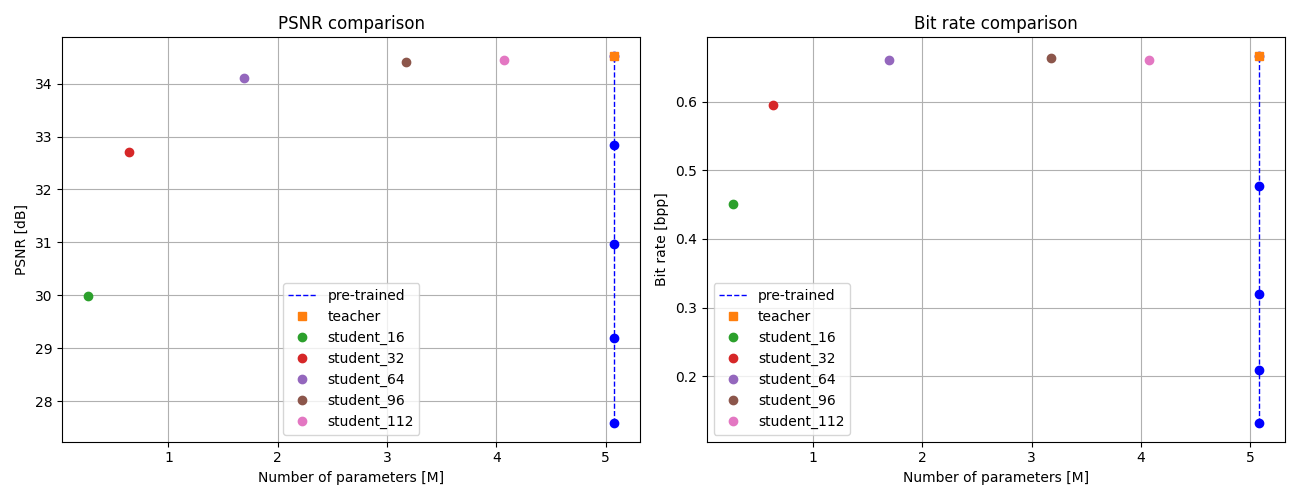
\includegraphics[width=15cm]{../img/kd_lic_parameters.png}
    \caption[\acrshort{psnr} and bit rate on the Kodak dataset according to students number of parameters.]{\acrshort{psnr} and bit rate on the Kodak dataset according to students number of parameters. Reducing the number of parameters graduatly decrease \acrshort{rd} results. Similar results are observed for memory footprint. In our testing, a fair balance between \acrshort{rd} and memory footprint is using 64 channels as it virtually does not degrade performance while reducing the memory footprint by 68 \%.}
    \label{kd_lic_parameters}
\end{figure}

\begin{table}[]
    \centering
    \caption[Number of parameters, memory footprint, \acrshort{psnr} and bit rate for teacher and student models.]{Number of parameters, memory footprint, \acrshort{psnr} and bit rate for teacher and student models.}
    \label{tab_size}
    \begin{tabular}{|c|c|lr|lr|lr|lr|}
        \hline
        Model                    & \begin{tabular}[c]{@{}c@{}}Number\\ of channels\end{tabular} & \multicolumn{2}{c|}{\begin{tabular}[c]{@{}c@{}}Number of\\ parameters {[}M{]}\end{tabular}} & \multicolumn{2}{c|}{\begin{tabular}[c]{@{}c@{}}Memory\\ footprint {[}MB{]}\end{tabular}} & \multicolumn{2}{c|}{PSNR} & \multicolumn{2}{c|}{\begin{tabular}[c]{@{}c@{}}Bit rate\\ {[}bpp{]}\end{tabular}} \\ \hline
        Teacher                  & 128                                                          & {\color[HTML]{656565} }                          & 5.08                                     & {\color[HTML]{656565} }                        & 20.18 & {\color[HTML]{656565} }          & 34.53 & {\color[HTML]{656565} }          & 0.67 \\ \hline
        \multirow{5}{*}{Student} & 112                                                          & {\color[HTML]{656565} -19.77 \%}                 & 4.07                                     & {\color[HTML]{656565} -23.03 \%}               & 15.53 & {\color[HTML]{656565} -0.26 \%}  & 34.44 & {\color[HTML]{656565} -1.03 \%}  & 0.66 \\ \cline{2-10} 
                                 & 96                                                           & {\color[HTML]{656565} -37.47 \%}                 & 3.17                                     & {\color[HTML]{656565} -40.01 \%}               & 12.11 & {\color[HTML]{656565} -0.33 \%}  & 34.41 & {\color[HTML]{656565} -0.58 \%}  & 0.66 \\ \cline{2-10} 
                                 & 64                                                           & {\color[HTML]{656565} -66.62 \%}                 & 1.69                                     & {\color[HTML]{656565} -67.98 \%}               & 6.46  & {\color[HTML]{656565} -1.21 \%}  & 34.11 & {\color[HTML]{656565} -0.91 \%}  & 0.66 \\ \cline{2-10}
                                 & 32                                                           & {\color[HTML]{656565} -87.46 \%}                 & 0.64                                     & {\color[HTML]{656565} -87.97 \%}               & 2.43  & {\color[HTML]{656565} -5.25 \%}  & 32.71 & {\color[HTML]{656565} -10.73 \%} & 0.60 \\ \cline{2-10} 
                                 & 16                                                           & {\color[HTML]{656565} -94.77 \%}                 & 0.27                                     & {\color[HTML]{656565} -94.98 \%}               & 1.01  & {\color[HTML]{656565} -13.17 \%} & 29.98 & {\color[HTML]{656565} -32.44 \%} & 0.45 \\ \hline
    \end{tabular}
\end{table}

Computers can only perform a certain amount of operations per unit of time. When using with mainstream hardware, the computing power required to use an image compression model like the scale hyperprior model is sufficient. However, when dealing with resource constrained devices, the latency might increase which goes against the objective of real-time decompression. With too much latency, it is impossible too extend image decompression to video decompression. Here, we focus on two metrics: the number of \acrfull{flop}s (i.e. the number of floating-point operations carried out to run an inference) and the model throughput (i.e. the number of frames that can process the model in one second). According to our results, the student with 16 channels only requires 3 \% of the teacher \acrshort{flop}s to perform the inference which translates to a 25 \% increase in throughput (Table \ref{tab_compute}). Figures \ref{kd_lic_flop} and \ref{kd_lic_fps} show that once again, the student with 64 channels represents the best compromise between \acrshort{rd} and \acrshort{flop}s or throughput. It should also be noted that all our models present a throughput that exceeds all requirements for video streaming. This headroom can be used in different ways: we can either increase the stream resolution to enhance user experience or reduce the inference frequency to save energy. 

\begin{figure}
    \centering
    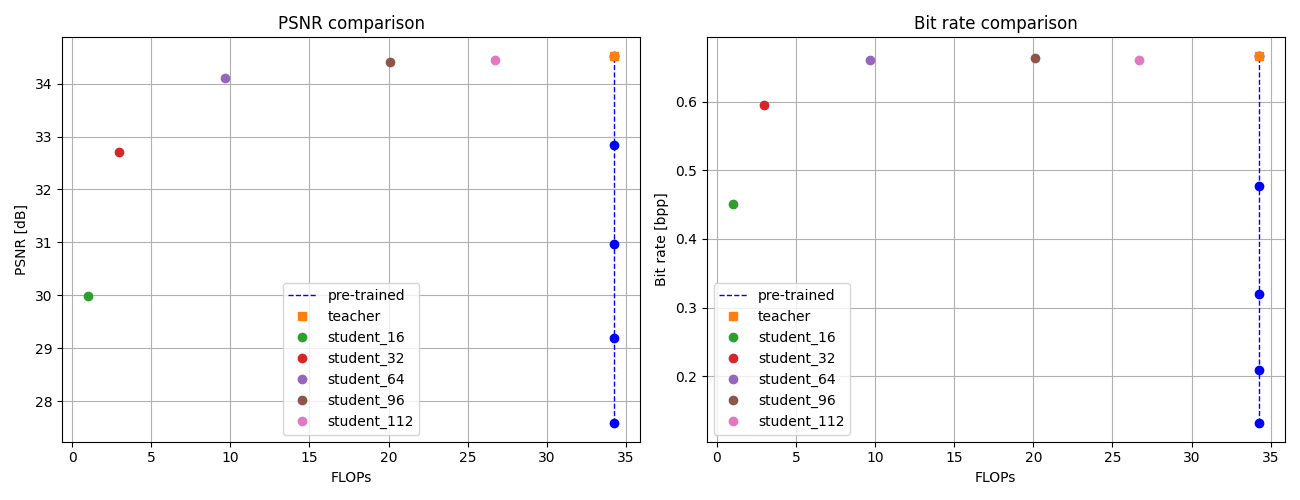
\includegraphics[width=15cm]{../img/kd_lic_flop.png}
    \caption[\acrshort{psnr} and bit rate on the Kodak dataset according to students \acrshort{flop}s.]{\acrshort{psnr} and bit rate on the Kodak dataset according to students \acrshort{flop}s. Our knowledge distilled models are good candidates for devices with limited compute power. They all offer lower \acrshort{flop} counts than standard models. However, this comes at a non-negligeable cost in image quality and bit rate for the smallest models.}
    \label{kd_lic_flop}
\end{figure}

\begin{figure}
    \centering
    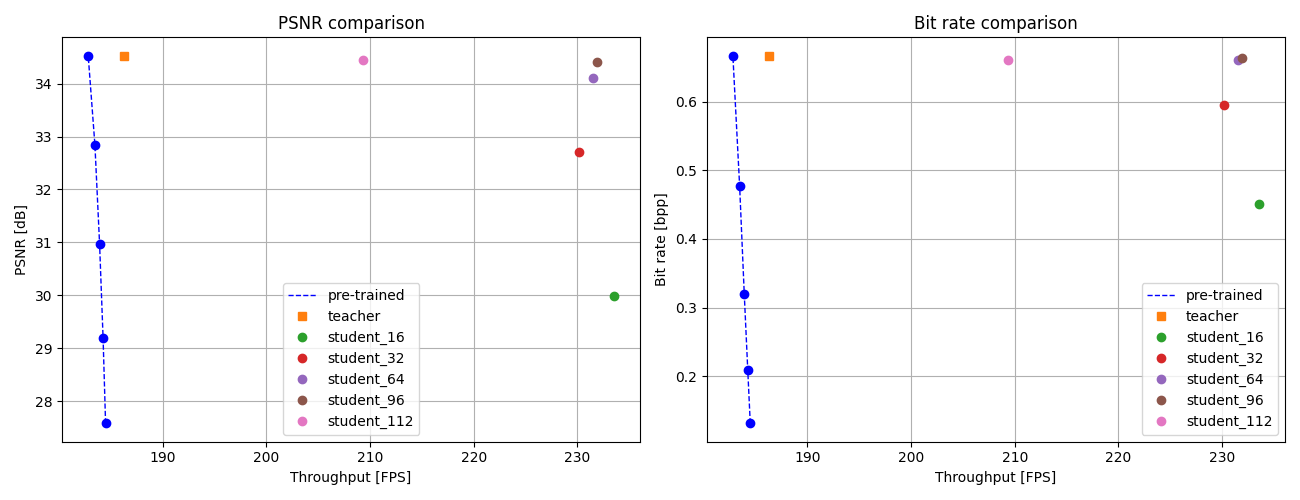
\includegraphics[width=15cm]{../img/kd_lic_fps.png}
    \caption[\acrshort{psnr} and bit rate on the Kodak dataset according to students throughput.]{\acrshort{psnr} and bit rate on the Kodak dataset according to students throughput. All models, exceed standard frame rate. With, higher throughput than pre-trained models, our knowledge distilled models have more headroom for higher resolution frames or lower energy consumption depending the real world application.}
    \label{kd_lic_fps}
\end{figure}

\begin{table}[]
    \centering
    \caption[\acrshort{flop}s, throughput, \acrshort{psnr} and bit rate for teacher and student models.]{\acrshort{flop}s, throughput, \acrshort{psnr} and bit rate for teacher and student models.}
    \label{tab_compute}
    \begin{tabular}{|c|c|lr|lr|lr|lr|}
    \hline
    Model                    & \begin{tabular}[c]{@{}c@{}}Number\\ of channels\end{tabular} & \multicolumn{2}{c|}{\begin{tabular}[c]{@{}c@{}}Floating point\\ operations\\ {[}GFLOP/frame{]}\end{tabular}} & \multicolumn{2}{c|}{\begin{tabular}[c]{@{}c@{}}Throughput\\ {[}FPS{]}\end{tabular}} & \multicolumn{2}{c|}{PSNR} & \multicolumn{2}{c|}{\begin{tabular}[c]{@{}c@{}}Bit rate\\ {[}bpp{]}\end{tabular}} \\ \hline
    Teacher                  & 128                                                          & {\color[HTML]{656565} }                                & 34.24                                             & {\color[HTML]{656565} }                     & 184.20 & {\color[HTML]{656565} }          & 34.53 & {\color[HTML]{656565} }          & 0.67 \\ \hline
    \multirow{5}{*}{Student} & 112                                                          & {\color[HTML]{656565} -22.01 \%}                       & 26.70                                             & {\color[HTML]{656565} +13.47 \%}            & 209.01 & {\color[HTML]{656565} -0.26 \%}  & 34.44 & {\color[HTML]{656565} -1.03 \%}  & 0.66 \\ \cline{2-10} 
                             & 96                                                           & {\color[HTML]{656565} -41.31 \%}                       & 20.10                                             & {\color[HTML]{656565} +25.74 \%}            & 231.61 & {\color[HTML]{656565} -0.33 \%}  & 34.41 & {\color[HTML]{656565} -0.58 \%}  & 0.66 \\ \cline{2-10}
                             & 64                                                           & {\color[HTML]{656565} -71.75 \%}                       & 9.67                                              & {\color[HTML]{656565} +26.20 \%}            & 232.47 & {\color[HTML]{656565} -1.21 \%}  & 34.11 & {\color[HTML]{656565} -0.91 \%}  & 0.66 \\ \cline{2-10} 
                             & 32                                                           & {\color[HTML]{656565} -91.31 \%}                       & 2.98                                              & {\color[HTML]{656565} +25.89 \%}            & 231.90 & {\color[HTML]{656565} -5.25 \%}  & 32.71 & {\color[HTML]{656565} -10.73 \%} & 0.60 \\ \cline{2-10}
                             & 16                                                           & {\color[HTML]{656565} -97.01 \%}                       & 1.02                                              & {\color[HTML]{656565} +26.83 \%}            & 233.63 & {\color[HTML]{656565} -13.17 \%} & 29.98 & {\color[HTML]{656565} -32.44 \%} & 0.45 \\ \hline
    \end{tabular}
\end{table}

Most edge devices also have access to a limited amount of energy whether it is in time because they run on battery like smartphones or because they are \acrfull{iot} devices that run 24/7 and thus should not consume a lot of energy. This is why we focus on the energy required to process a single frame. Table \ref{tab_energy} shows that we can save up to 60 \% of the energy used by the teacher model by using the student with 16 channels. Using Figure \ref{kd_lic_energy}, that the model that offers the best tradeoff between \acrshort{psnr} and energy consumption in the student model with 64 channels. By using this model we keep the same image quality while reducing our energy consumption by 35 \%.

\begin{figure}
    \centering
    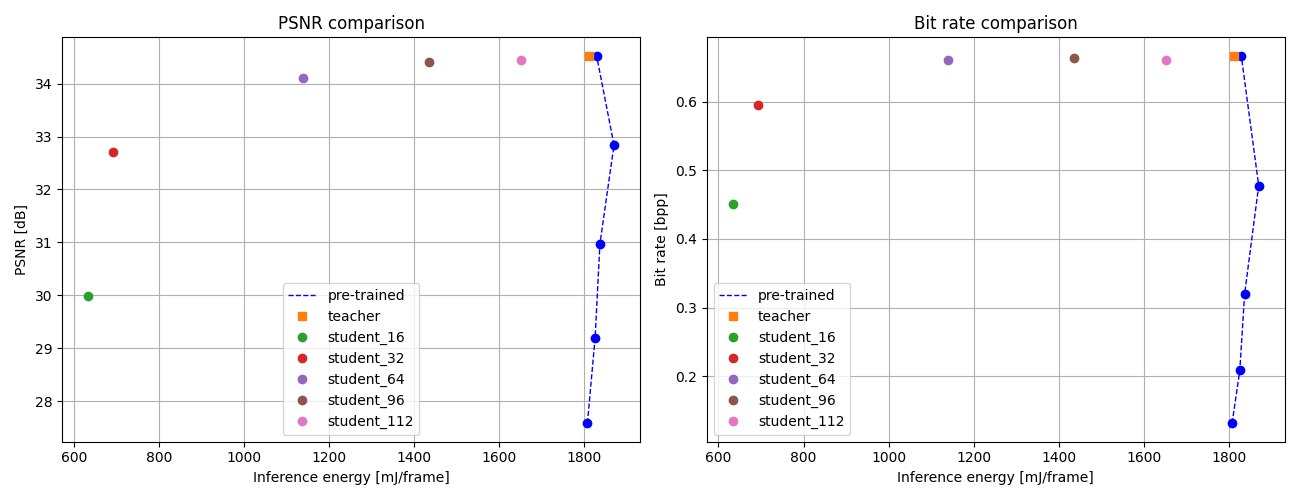
\includegraphics[width=15cm]{../img/kd_lic_energy.png}
    \caption[\acrshort{psnr} and bit rate on the Kodak dataset according to students consumed energy.]{\acrshort{psnr} and bit rate on the Kodak dataset according to students consumed energy. \acrshort{kd} is a great method to create energy friendly \acrshort{lic} models. If energy consumption is not too restricted, we recommand using the student with 64 channels that consumes 35 \% less energy per frame and achieve image compression on par with the teacher model.}
    \label{kd_lic_energy}
\end{figure}

\begin{table}[]
    \centering
    \caption[Consumed energy, \acrshort{psnr} and bit rate for teacher and student models.]{Consumed energy, \acrshort{psnr} and bit rate for teacher and student models.}
    \label{tab_energy}
    \begin{tabular}{|c|c|lr|lr|lr|}
        \hline
        Model                    & \begin{tabular}[c]{@{}c@{}}Number\\ of channels\end{tabular} & \multicolumn{2}{c|}{\begin{tabular}[c]{@{}c@{}}Energy\\ {[}mJ/frame{]}\end{tabular}} & \multicolumn{2}{c|}{PSNR} & \multicolumn{2}{c|}{\begin{tabular}[c]{@{}c@{}}Bit rate\\ {[}bpp{]}\end{tabular}} \\ \hline
        Teacher                  & 128                                                          & {\color[HTML]{656565} }                     & 1767.85 & {\color[HTML]{656565} }          & 34.53 & {\color[HTML]{656565} }          & 0.67 \\ \hline
        \multirow{5}{*}{Student} & 112                                                          & {\color[HTML]{656565} -9.47 \%}             & 1600.41 & {\color[HTML]{656565} -0.26 \%}  & 34.44 & {\color[HTML]{656565} -1.03 \%}  & 0.66 \\ \cline{2-8} 
                                 & 96                                                           & {\color[HTML]{656565} -19.88 \%}            & 1416.34 & {\color[HTML]{656565} -0.33 \%}  & 34.41 & {\color[HTML]{656565} -0.58 \%}  & 0.66 \\ \cline{2-8}
                                 & 64                                                           & {\color[HTML]{656565} -34.15 \%}            & 1164.17 & {\color[HTML]{656565} -1.21 \%}  & 34.11 & {\color[HTML]{656565} -0.91 \%}  & 0.66 \\ \cline{2-8}
                                 & 32                                                           & {\color[HTML]{656565} -60.45 \%}            & 699.18  & {\color[HTML]{656565} -5.25 \%}  & 32.71 & {\color[HTML]{656565} -10.73 \%} & 0.60 \\ \cline{2-8}
                                 & 16                                                           & {\color[HTML]{656565} -61.28 \%}            & 684.45  & {\color[HTML]{656565} -13.17 \%} & 29.98 & {\color[HTML]{656565} -32.44 \%} & 0.45 \\ \hline
    \end{tabular}
\end{table}

In order to put our results into context, we also measured throughput, energy consumption, \acrshort{psnr} and bit rate for three image compression codecs, namely: JPEG-2000, JPEG and WepP. The first row of Table \ref{tab_energy} shows that JPEG-2000 is not suited for our application due to its emphasis on image quality. The bit rate and energy consumption are to high. In addition to this, the throughput is very low making it unusable in real-time. Our experiments show that studied \acrshort{lic} models outperform JPEG and WepP in \acrshort{rd} (Figure \ref{appendix:codecs_rd}). Both JPEG and WepP could be used in real-time albeit at a lower frame rate than our \accrhort{nn}s (Figure \ref{appendix:codecs_fps}). However, when it comes to energy consumption, the superiority of \acrshort{lic} models is challenged: JPEG achieves better \acrshort{psnr} and bit rate with less energy (Figure \ref{appendix:codecs_energy}). This brief comparison with traditional codecs show that \acrshort{lic} models, and especially our distilled models, are relevant candidates for real-time image compression on resource constrained platforms. These models propose an interesting compromise between throughput, energy consumption and quality of image compression.

\begin{table}[]
    \centering
    \caption[Throughput, consumed energy, \acrshort{psnr} and bit rate for different codecs.]{Consumed energy, \acrshort{psnr} and bit rate for different codecs.}
    \label{tab_codecs}
    \begin{tabular}{|c|r|r|r|r|}
        \hline
        Codec                  & \multicolumn{1}{c|}{\begin{tabular}[c]{@{}c@{}}Throughput\\ {[}FPS{]}\end{tabular}} & \multicolumn{1}{c|}{\begin{tabular}[c]{@{}c@{}}Energy\\ {[}mJ/frame{]}\end{tabular}} & \multicolumn{1}{c|}{PSNR}                            & \multicolumn{1}{c|}{\begin{tabular}[c]{@{}c@{}}Bit rate\\ {[}bpp{]}\end{tabular}} \\ \hline
        JPEG 2000              & 10.15                                                                               & 2308.87                                                                              & 70.0                                                 & 13.45                                                                             \\ \hline
                               & 130.12                                                                              & \cellcolor[HTML]{32CB00}185.84                                                       & 26.65                                                & 0.33                                                                              \\ \cline{2-5} 
                               & \cellcolor[HTML]{32CB00}134.30                                                      & \cellcolor[HTML]{CB0000}804.04                                                       & \cellcolor[HTML]{CB0000}21.41                        & \cellcolor[HTML]{32CB00}0.17                                                      \\ \cline{2-5} 
        \multirow{-3}{*}{JPEG} & \cellcolor[HTML]{CB0000}86.51                                                       & 274.94                                                                               & \cellcolor[HTML]{32CB00}{\color[HTML]{333333} 40.55} & \cellcolor[HTML]{CB0000}3.40                                                      \\ \hline
                               & \cellcolor[HTML]{CB0000}19.11                                                       & 1216.75                                                                              & 43.03                                                & 3.85                                                                              \\ \cline{2-5} 
                               & \cellcolor[HTML]{32CB00}39.61                                                       & 603.38                                                                               & 25.85                                                & 0.11                                                                              \\ \cline{2-5} 
                               & 39.56                                                                               & \cellcolor[HTML]{32CB00}{\color[HTML]{333333} 595.61}                                & \cellcolor[HTML]{CB0000}25.85                        & \cellcolor[HTML]{32CB00}0.11                                                      \\ \cline{2-5} 
                               & 19.12                                                                               & 1220.86                                                                              & \cellcolor[HTML]{32CB00}43.03                        & \cellcolor[HTML]{CB0000}3.85                                                      \\ \cline{2-5} 
        \multirow{-5}{*}{WepP} & 19.14                                                                               & \cellcolor[HTML]{CB0000}1232.84                                                      & 43.03                                                & 3.85                                                                              \\ \hline
    \end{tabular}
\end{table}

This section is a deep dive into the resource consumption of standard and knowledge distilled models. Based on measures of memory usage, required computing power and energy consumption on students architectures with varying number of channels, we prove that \acrshort{kd} indeed create frugal models. In all experiments, our \acrshort{kd} models consume less resources that standard models at a (sometimes negligeable) cost in \acrshort{rd} performance. On a not-too-constrained platform, we would recommand the use of the student with 64 channels. It has a limited use of resources without noticeable impact on image compression.

This chapter is a step in the right direction for \acrshort{lic} on resource constrained platforms. We first assess the effectiveness of \acrshort{kd} on well known models and tasks then transfer this frugal \acrshort{ai} technique to \acrshort{lic}. \acrshort{rd} results are impressive, showing models with as low as half as many channels in the same operational region as their teacher. We also experiment with different teachers and find that we can train student models adapted for any image compression/resource consumption tradeoff possible. Other settings like the loss function definitely impact the student performances, leaving room for other research work. Most importantly, we measure a significant reduction in the model resource consumption (memory, compute, and energy) without too much degradation of the image compression \acrshort{rd}. We observe that \acrshort{kd} is a valuable training paradigm in order to achieve real-time image compression on resource limited devices.